\documentclass[11pt,a4paper]{report} 
% Alternativ für doppelseitigen Ausdruck (nur bei > 60 Seiten sinnvoll)
% \documentclass[11pt,a4paper,twoside,openright]{report} 

% Deutsch
%\usepackage[german]{babel} % deutsch und deutsche Rechtschreibung
%\usepackage[english]{babel}
\usepackage[main=english, german]{babel}
\usepackage[utf8]{inputenc} % Unicode Text 
\usepackage[T1]{fontenc} % Umlaute und deutsches Trennen
\usepackage{textcomp} % Euro
\usepackage[hyphens]{url}
% statt immer Ab\-schluss\-ar\-beit zu schreiben
% einfach hier sammeln mit -. 
\hyphenation{Ab-schluss-ar-beit}
% Vorsicht bei Umlauten und Bindestrichen
\hyphenation{Ver-st\"ar-ker-aus-gang}
 % eigene Hyphenations, die für das Dokument gelten
\usepackage{amssymb} % Symbole
\usepackage{emptypage} % Wirklich leer bei leeren Seiten


%% Fonts, ein kompletter Satz an Optionen

% Times New Roman, gewohnter Font, ok tt und serifenlos
%\usepackage{mathptmx} 
%\usepackage[scaled=.95]{helvet}
%\usepackage{courier}

% Palatino mit guten Fonts für tt und serifenlos
\usepackage{mathpazo} % Palatino, mal was anderes
\usepackage[scaled=.95]{helvet}
\usepackage{courier}

% New Century Schoolbook sieht auch nett aus (macht auch tt und serifenlos)
%\usepackage{newcent}

% Oder default serifenlos mit Helvetica 
% ich kann es nicht mehr sehen ...
%\renewcommand{\familydefault}{\sfdefault}

\usepackage{microtype}

% Bilder und Listings
\usepackage{graphicx} % wir wollen Bilder einfügen
\usepackage{subfig} % Teilbilder
\usepackage{wrapfig} % vielleicht doch besser vermeiden
\usepackage{listings} % schöne Quellcode-Listings
% ein paar Einstellungen für akzeptable Listings
\lstset{basicstyle=\ttfamily, columns=[l]flexible, mathescape=true, showstringspaces=false, numbers=left, numberstyle=\tiny}
\lstset{language=python} % und nur schöne Programmiersprachen ;-)
% und eine eigene Umgebung für Listings
\usepackage{float}
\newfloat{listing}{htbp}{scl}[chapter]
\floatname{listing}{Listing}

% Seitenlayout
\usepackage[paper=a4paper,width=14cm,left=35mm,height=22cm]{geometry}
\usepackage{setspace}
\linespread{1.15}
\setlength{\parskip}{0.5em}
\setlength{\parindent}{0em} % im Deutschen Einrückung nicht üblich, leider

% Seitenmarkierungen 
\newcommand{\phv}{\fontfamily{phv}\fontseries{m}\fontsize{9}{11}\selectfont}
\usepackage{fancyhdr} % Schickere Header und Footer
\pagestyle{fancy}
\renewcommand{\chaptermark}[1]{\markboth{#1}{}}
%\fancyhead[L]{\phv \leftmark}
\fancyhead[L]{\phv \nouppercase{\leftmark}}
\fancyhead[R]{\phv \thepage}
% Unten besser auf alles Verzichten
%\fancyfoot[L]{\textsf{\small \kurztitel}}
\fancyfoot[C]{\ } % keine Seitenzahl unten
%\fancyfoot[R]{\textsf{\small Medieninformatik}}

% Theorem-Umgebungen
\newtheorem{definition}{Definition}[chapter]
\newtheorem{satz}{Satz}[chapter]
\newtheorem{lemma}[satz]{Lemma} % gleicher Zähler wie Satz
\newtheorem{theorem}{Theorem}[chapter]
\newenvironment{beweis}[1][Beweis]{\begin{trivlist}
\item[\hskip \labelsep {\textit{#1 }}]}{\end{trivlist}}
\newcommand{\qed}{\hfill \ensuremath{\square}}

% Quellen teilen
\usepackage{bibtopic} 

% Hochschule Logo, noch nicht perfekt
\usepackage{hsrmlogo}

% Spezialpakete
\usepackage{epigraph}
\setlength{\epigraphrule}{0pt} % kein Trennstrich

% damit wir nicht so viel tippen müssen, nur für Demo 
\usepackage{blindtext} 

% Zum Zeigen von Fehlern
\usepackage{soul}
\newcommand*\falsch{\st}

 % alle Pakete und Einstellungen

% Hier anpassen 
\newcommand{\welchethesis}{Bachelor}
% \newcommand{\welchethesis}{Master}
\newcommand{\thesisofwas}{of Science - B.Sc.}
\newcommand{\titel}{Study and implementation of a decentralized application that can provide
	permissionless financial services using an evm based blockchain}
%\newcommand{\kurztitel}{Template Abschlussarbeit}
\newcommand{\autor}{Mario Alberto Maita Orozco}
\newcommand{\datum}{30.06.2022} % Abgabedatum
\newcommand{\ort}{Wiesbaden}
\newcommand{\referent}{Prof.\ Dr.\ Eva-Maria Iwer}
\newcommand{\korreferent}{Prof.\ Dr.\ Marc-Alexander Zschiegner}

\begin{document}

\begin{titlepage}
  \begin{center}
    % Kopf der Seite
    \hsrmlogo[1]
    \parbox[b]{8cm}{Hochschule RheinMain \\
     Fachbereich Design Informatik Medien \\
     Studiengang Informatik - Technische Systeme}
    \vfill    
    {\LARGE Bachelor-Arbeit} \\[0.5cm]
    {\large zur Erlangung des akademischen Grades} \\[5mm]
    {\large \welchethesis\ \thesisofwas} \\[5mm]
    \rule{\textwidth}{1pt}\\[0.5cm]
    {\begin{spacing}{1.15} \LARGE \bfseries \titel \\ \end{spacing}}
    \rule{\textwidth}{1pt}    
    \vfill    
    \begin{tabular}{ll} % Mitte der Seite
      Vorgelegt von & \autor \\
      am & \datum \\
      Referent & \referent \\
      Korreferent & \korreferent
    \end{tabular}    
    \vfill
  \end{center}
\end{titlepage}
\cleardoublepage


% Erklärung gemäß den Allgemeinen Bestimmungen für Prüfungsordnungen
% der Paragraph schwankt, daher ohne Nennung einer Nummer
\thispagestyle{empty}
\section*{Erklärung gem. ABPO, Ziff. 4.1.5.4}
Ich versichere, dass ich die Bachelor-Arbeit selbständig verfasst und keine anderen als
die angegebenen Hilfsmittel benutzt habe.
´

\vspace{6em}
\noindent\begin{tabular}{p{0.37\textwidth}p{0.56\textwidth}}
\ort, \datum  & \rule{0.56\textwidth}{0.5pt}\\
              & \makebox[1cm]{\ } \autor
\end{tabular}

\vfill

\section*{Erklärung zur Verwendung der \welchethesis thesis}

Hiermit erkläre ich mein Einverständnis mit den im Folgenden aufgeführten
Verbreitungsformen dieser Bachelor-Arbeit:

\vspace{1em}
\noindent\begin{tabular}{|p{0.82\textwidth}|c|c|}
  \hline
  \textbf{Verbreitungsform} & \makebox[0.035\textwidth]{\textbf{Ja}} 
                            & \makebox[0.05\textwidth]{\textbf{Nein}} \\\hline
  Einstellung der Arbeit in die Hochschulbibliothek 
                         mit Datenträger   &  & $\times$ \\\hline
  Einstellung der Arbeit in die Hochschulbibliothek  
                         ohne Datenträger  & $\times$ & \\\hline
  Veröffentlichung des Titels der Arbeit im Internet  
                                           & $\times$ & \\\hline
  Veröffentlichung der Arbeit im Internet             
                                           &  $\times$  & \\\hline
\end{tabular}

\vspace{6em}
\noindent\begin{tabular}{p{0.37\textwidth}p{0.56\textwidth}}
\ort, \datum  & \rule{0.56\textwidth}{0.5pt}\\
              & \makebox[1cm]{\ } \autor
\end{tabular}
\cleardoublepage

 % Titelseite, Erklärungen, etc.

\begin{abstract} 
\LaTeX\ bietet Buchdruckqualität für jedermann.
Wir zeigen anhand dieses durch persönliche Präferenzen geprägtes Template, 
wie man Buchdruckqualität für eine Abschlussarbeit einfach erreichen kann.
Dazu werden beispielhaft Lösungen zu üblichen Fragestellungen im Dokument 
vorgestellt.
Zunächst benötigt man ein passendes \LaTeX\ System mit einigen 
installierten Erweiterungspaketen, das es erlaubt das Template zu 
übersetzen. 
Neben den grundlegenden For\-ma\-tie\-rungs\-möglich\-keiten mit \LaTeX\ wird 
insbesondere das Erstellen und Einbinden von Grafiken, Listings und 
mathematischen Formeln gezeigt.
Des Weiteren werden Literatur- und andere Verzeichnisse eingebunden.
Nicht zuletzt finden sich auch sachdienliche Hinweise zum
Schreiben und Zitieren von Literatur.
\end{abstract}

\tableofcontents
\newpage 

\chapter{Introduction} \label{ch:intro}
%\epigraphhead[70]{\epigraph{Documentation is like sex: 
%when it is good, it is very, very good; and when it is bad, 
%sit is better than nothing.}{\textit{Dick Brandon}}}

Example refering a label:   in chapter ~\ref{ch:intro}

\section{Motivation}
\section{Goals}
\section{Thesis Structure}
The Thesis is divided into the following chapters:
\begin{itemize}
	\item \textbf{Chapter~\ref{ch:background}} ...
	\item \textbf{Chapter~\ref{ch:background}} ...
	\item \textbf{Chapter~\ref{ch:background}} ...
	\item \textbf{Chapter~\ref{ch:background}} ...
	\item \textbf{Chapter~\ref{ch:background}} ...
\end{itemize}


%%%%%
%%%%% Chapter
\chapter{Background} \label{ch:background}

\section{Blockchain} \label{}
\subsection{Cryptography}
\subsubsection{Cryptographic hash functions}
\subsubsection{Merkle tree}
\subsection{Consensus Mechanism}
\subsection{Bitcoin}
\section{Ethereum}
\subsection{Ethereum Virtual Machine (EVM)}
\subsection{Smart Contracts}
\subsection{Decentralized Applications (Dapps)}

\begin{table}
\centering
\begin{tabular}{|l||l|l|}
\hline
\multicolumn{1}{|c|}{\textbf{Plattform}} & 
\multicolumn{1}{|c|}{\textbf{\LaTeX-Distribution}} & 
\multicolumn{1}{|c|}{\textbf{Editor}} \\\hline\hline
Linux/Unix & TeX Live & Texmaker \\\hline
MacOSX     & TeX Live & Texmaker \\\hline
Windows    & MiKTeX   & Texmaker \\\hline   
\end{tabular}
\caption{\LaTeX-Distributionen und Editor je Plattform}
\label{tab:disteditplattform}
\end{table}





\begin{figure}[htp]
\centering
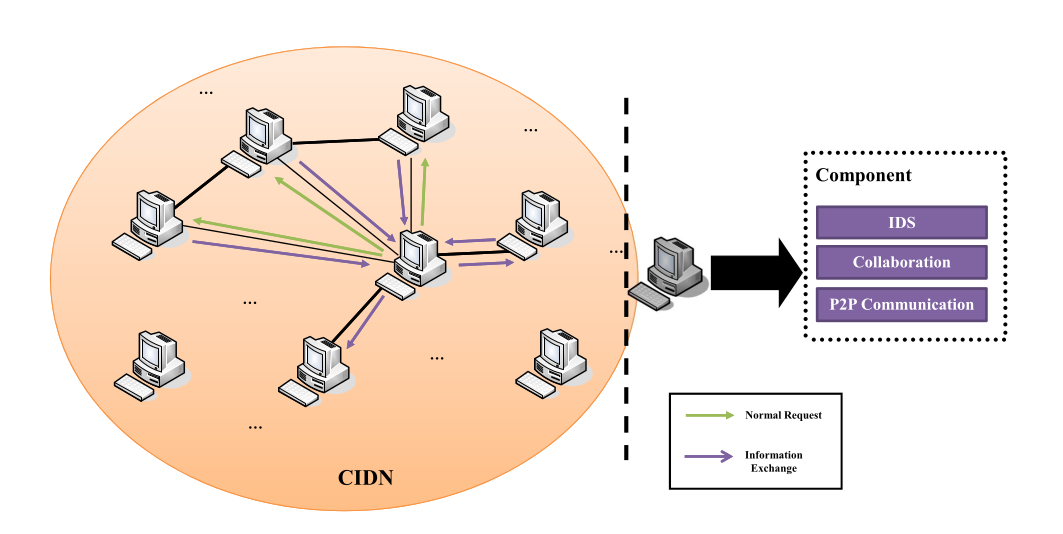
\includegraphics[width=.9\textwidth]{images/cids}
\caption{Dateien zur Erstellung des Templates}
\label{fig:templateprozess}
\end{figure}



%%%%%
%%%%% Chapter
\chapter{State of the Art, Protocols to be used} \label{}


%%%%%
%%%%% Chapter
\chapter{Application requirements} \label{}


\section{Listings} \label{sec:listings}

\begin{listing}[htbp]
\begin{lstlisting}
def ggt(x, y):
    while x != 0:
        x,y = y%x, x
    return y
\end{lstlisting}
\caption{ggT --- kurz und gut}
\label{code:ggt}
\end{listing}


%%%%%
%%%%% Chapter
\chapter{Implementation and testing} \label{chap:stil}



%%%%%
%%%%% Chapter
\chapter{Conclusion and future work} \label{ch:conclusion}

Mit \LaTeX\ die Abschlussarbeit zu schreiben ist 
einfach und ergibt ein schönes, hochqualitatives Dokument.
Die Umgebung ist kostenlos und steht auf allen wichtigen
Plattformen zur Verfügung.
Im Gegensatz zu anderen Tools kann man sich beim Schreiben 
auf den Inhalt konzentrieren und steht großen Änderungen 
nicht ängstlich gegenüber.

Die Stärken von \LaTeX\ sind das Schreiben des Fließtexts
durch die Angabe von Struktur. 
Referenzieren innerhalb des Dokuments und auch auf 
Literatur sind sehr einfach und vollständig automatisiert. 
Selbst wenn die Erstellung von Bildern innerhalb von
\LaTeX\ auch möglich ist, verwenden viele lieber externe 
Tools für die Grafiken und binden diese dann ein. 
Auch dies wird sehr gut unterstützt und diese und
weitere Elemente wie Listings und Tabellen werden
von \LaTeX\ an eine passende Stelle gesetzt.

Das vorliegende Template vereinfacht die Erstellung
einer Abschlussarbeit an der Hochschule~RheinMain,
da formale Vorgaben an eine solche Abschlussarbeit
umgesetzt sind. 
Darüber hinaus ist das Template jedoch geprägt von 
persönlichen Vorlieben des Referenten. 
Diese persönlichen Vorlieben können Sie jedoch 
nach eingehender Beschäftigung mit \LaTeX\ auch gerne 
anders ausgestalten und einen eigenen Stil entwickeln.

Happy \TeX ing! 

\newpage

% Listen wenn überhaupt ans Ende und nicht an den Anfang.
% Meist ist das aber unnötig.
%\listoffigures % Liste der Abbildungen 
%\listoftables % Liste der Tabellen
% \newpage

\bibliographystyle{plain} % Literaturverzeichnis
\begin{btSect}{thesis} % mit bibtopic Quellen trennen
\section*{Bibliography}
\btPrintCited
\end{btSect}
\begin{btSect}{online}
\section*{Online Sources}
\btPrintCited
\end{btSect}
% dann mit "bibtex thesis1" und "bibtex thesis2" arbeiten

\end{document}
;;; Local Variables:
;;; ispell-local-dictionary: "de_DE-neu"
;;; End:
